\chapter{ПРЕДЛАГАЕМОЕ РЕШЕНИЕ} \label{ch3}
Одной из основных целей данной работы было разработать графический конвейер, максимально приближенный к существующим графическим конвейерам. Таким образом будут достигнуты две цели:
\begin{enumerate}[1.] 
	\item Эксперименты, проводимые при помощи разработанной архитектуры, будут содержать те же затратные (с точки зрения производительности) места, которые имеют современные графические системы. А значит, результаты, полученные в ходе экспериментов, будут более приближены к значениям, получаемым в реальных современных графических системах
	\item Будут разработаны и реализованы алгоритмы, которые можно будет использовать другим графичеким системам, если они возмут за основу предлагаемую архитектуру
\end{enumerate}


\section{Непрямая отрисовка} \label{ch3:indirect_draw}
Как было уже упомянуто ранее, основным способом отправки команд на графический процессор считается сбор \say{списка команд} на центральном процессоре и последующая передача получившегося \say{списка} на графический процессор. Однако современных API добавилась возможность дополнить вышеупомянутый \say{список команд} дополнительным массивом команд прямо из графического процессора. Эта технология называется непрямой отрисовкой и в DirectX 12 эту технологию реализует команда ExecuteIndirect. 

Для того чтобы воспользоваться командой ExecuteIndirect, ей необходимо передать следующие параметры:
\begin{enumerate}[1.] 
	\item \say{Сигнатуру вызова} - перечень команд которые необходимо вызвать для каждого рисуемого объекта. Обязательно должна оканчиваться командой отрисовки.
	\item Буфер из видеопамяти с параметрами (которые требует сигнатура), для каждого выводимого объекта.
	\item Количество отрисовываемых объектов (число или указатель на буфер из видеопамяти).
\end{enumerate}

Таким образом, простейший алгоритм отрисовки любого числа объектов будет выглядеть так: (\firef{alg:simpleIndirect})

\begin{algorithm} %[h]
	\SetKwFunction{algoSimpleIndirectPseudocode}{} 
	\SetKwProg{myalg}{Algorithm}{}{} %write in 2nd agrument <<Algorithm>>, <<Procedure>> etc
	\nonl\myalg{\algoSimpleIndirectPseudocode}{
		Загрузить все объекты
		
		Создать сигнатуру
		
		Создать буфер (\textit{SRVbuffer}) и сохранить в него информацию для каждого объекта (например указатель на буфер вершин) 
		
		Установить формат хранения вершин
		
		Установить формат соединения вершин
		
		Установить программу-шейдер, для отрисовки
		
		
		\For {each frame}{
			ExecuteIndirect(\textit{SRVbuffer})
		}	
	}
	\caption{Примерный псевдокод простейшего алгоритма использующего непрямую отрисовку}\label{alg:simpleIndirect}
\end{algorithm}
\FloatBarrier

Таким образом мы добились поставленной цели, и количество команд в \say{списке команд} при данном подходе действительно константно относительно числа объектов. Но на практике этот алгоритм будет работать хуже, чем традиционный. Причина в том, что традиционный подход позволяет заранее отбросить отрисовку части объектов, просто не добавив их в \say{список команд}, а данный (\firef{alg:simpleIndirect}) алгоритм не даёт такой возможности. Однако, это можно было бы исправить, если буфер с параметрами (\textit{SRVbuffer}) мог бы изменяться на каждом кадре работы приложения. Это приводит нас к следующему алгоритму (\firef{alg:IndirectWithCull})

\begin{algorithm} %[h]
	\SetKwFunction{algoIndirectWithCullPseudocode}{} 
	\SetKwProg{myalg}{Algorithm}{}{} %write in 2nd agrument <<Algorithm>>, <<Procedure>> etc
	\nonl\myalg{\algoIndirectWithCullPseudocode}{
		Загрузить все объекты
		
		Создать сигнатуру
		
		Создать буфер (\textit{SRVbuffer}) и сохранить в него информацию для каждого объекта (например указатель на буфер вершин)
		
		Cоздать буфер (\textit{UAVbuffer}), совпадающий размером с предыдущим, 
		
		Cоздать счётчик (\textit{UAVcounter}) 
		
		Установить формат хранения вершин
		
		Установить формат соединения вершин
		
		\For {each frame}{
			
			Установить программу-шейдер, для обработки команд
			
			Обнулить счётчик (\textit{UAVcounter}) 
			
			Запустить вычислительный шейдер, который скопирует из \textit{SRVbuffer} в \textit{UAVbuffer} параметры нужных команд и изменит \textit{UAVcounter} на значение равное числу скопированных команд \label{alg:IndirectWithCull:culling}
			
			Установить программу-шейдер, для отрисовки
			
			ExecuteIndirect(\textit{UAVbuffer}, \textit{UAVcounter})
		}	
	}
	\caption{Примерный псевдокод алгоритма использующего непрямую отрисовку с отбрасыванием команд}\label{alg:IndirectWithCull}
\end{algorithm}
\FloatBarrier

Отметим преимущества и недостатки описанного алгоритма(\firef{alg:IndirectWithCull}):
\begin{enumerate}[1.] 
	\item Преимущество: число вызовов отрисовки в "списке команд" всё ещё является константным, относительно числа объектов
	\item Преимущество: число вызовов отрисовки на графическом процессоре не меняется(см главу \ref{ch2:Programmable-Vertex-Pulling})
	\item Преимущество: используются стандартные буферы, а значит оптимизации программы-драйвера не перестанут работать (см главу \ref{ch2:Programmable-Vertex-Pulling})
	\item Преимущество: нет проблем с фрагментацией (см главу \ref{ch2:Programmable-Vertex-Pulling})
	\item Преимущество: проверки проводимые при определении \say{нужных} команд (см \ref{alg:IndirectWithCull:culling} на \firef{alg:IndirectWithCull}), будут происходить параллельно. А так как обычно графический процессор обладает большим числом вычислительных ядер, чем центральный процессор, предложенный алгоритм будет работать быстрее.
	\item Недостаток: невозможно установить порядок, в котором объекты будут отрисовываться.
\end{enumerate} % Неявная отрисовка
\section{Общая структура} \label{ch3:pipeline_struct}
	Большинство графических приложений имеют схожую структуру конвейера отрисовки, состоящую из 3-х этапов:
	\begin{enumerate}[1.] 
		\item этап Pre-pass - выполнение задач, которые необходимо выполнить до рисования объектов на экран. Например: отбрасывание не видимых объектов, построение карт теней, предварительный подсчёт карты глубины.
		\item этап Render pass - отрисовка всех объектов на кадр.
		\item этап Post process - применение эффектов на получившийся кадр.
	\end{enumerate}
		
	\begin{figure}[ht!] 
		\center
		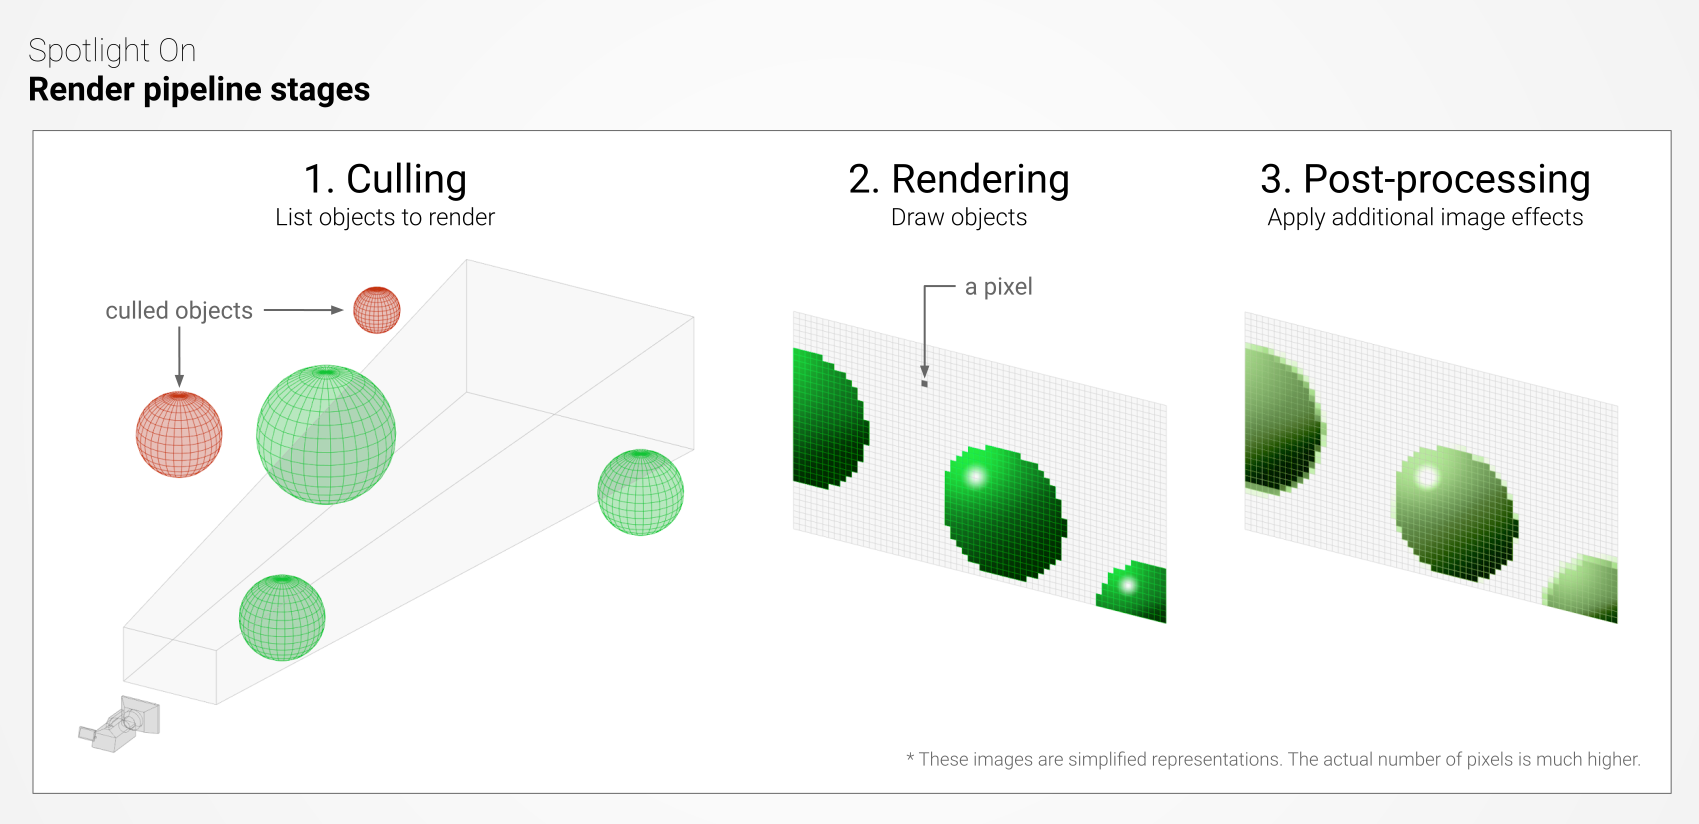
\includegraphics [scale=0.35] {my_folder/images//unity_pipeline}	
		\caption{Упрощенная схема конвейера отрисовки Unity} 
		\label{fig:unity_pipeline}  
	\end{figure}

	Предлагаемый конвейер сохраняет эту структуру, несмотря на изменения в алгоритме отрисовки, и требует 11 + S (где S - число источников света, отбрасывающих тень) вызовов отрисовки в \say{списке команд}, что видно по схеме конвейера на \firef{fig:pipeline_schema}. Каждый этап предствляет собой набор из подэтапов, где каждый подэтап решает ровно одну задачу.
	
	\begin{figure}[ht!] 
		\center
		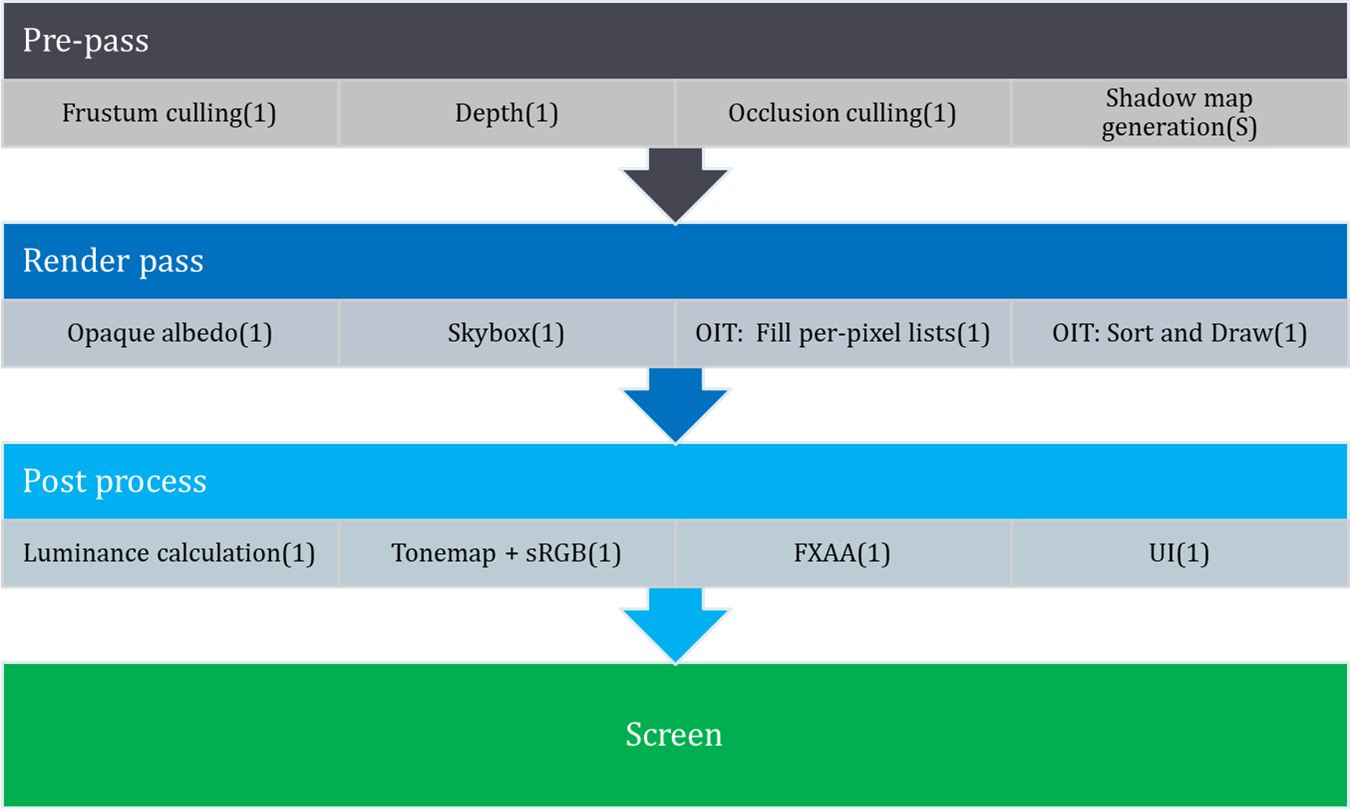
\includegraphics [scale=0.4] {my_folder/images//pipeline_schema}	
		\caption{Схема предлагаемого конвейера. В скобках указано количество вызывов ExecuteIndirect.} 
		\label{fig:pipeline_schema}  
	\end{figure}
	
	\FloatBarrier % Общая структура
\section{Этап Pre-pass} \label{ch3:pre_pass}
	\begin{figure}[ht!] 
		\center
		
\includegraphics [scale=0.4] {my_folder/images//prepass_schema}	
		\caption{Схема этапа Pre-pass предлагаемого конвеера.} 
		\label{fig:prepass_schema}
	\end{figure}
	
	На данном этапе реализуется отбрасывание команд и наполнение буфера, требуемого для выполнения команды ExecuteIndirect. Однако на одном и том же кадре могут требоваться команды, удовлетворяющие разным критериям, поэтому вводится несколько буферов, каждый из которых имеет разное имя
	\begin{enumerate}[1.]
		\item All
		\item OpaqueAll
		\item TransparentsAll
		\item OpaqueFrustum
		\item OpaqueCulled
		\item TransparentCulled
	\end{enumerate}

	\subsection{Frustum culling} \label{ch3:pre_pass:frustum}
	\subsection{Depth pre-pass} \label{ch3:pre_pass:depth}
	\subsection{Occlusion culling} \label{ch3:pre_pass:occlusion}
	\subsection{Построение карт теней} \label{ch3:pre_pass:shadow_maps} % Prepass	

\section{Этап Render pass} \label{ch3:render_pass}
	\subsection{Непрозрачные объекты} \label{ch3:render_pass:opaque}
		\subsubsection{Physically based render} \label{ch3:render_pass:opaque:pbr}
		\subsubsection{Image based lighting} \label{ch3:render_pass:opaque:ibl}
	\subsection{Skybox} \label{ch3:render_pass:skybox}
	\subsection{Полу-прозрачные объекты} \label{ch3:render_pass:transparents}
		\subsubsection{Order Independent Transparency} \label{ch3:render_pass:transparents:oit}
		\subsubsection{Weighted Blended Order Independent Transparency} \label{ch3:render_pass:transparents:wboit}
		\subsubsection{Hybrid Order Independent Transparency} \label{ch3:render_pass:transparents:hybrid_oit}
		
\section{Этап Post-process} \label{ch3:post_process}
	\subsection{Tonemapping, HDR и LDR} \label{ch3:post_process:hdr_ldr_tonemapping}
\section{Выводы} \label{ch3:conclusion}

%% Вспомогательные команды - Additional commands
%
%\newpage % принудительное начало с новой страницы, использовать только в конце раздела
%\clearpage % осуществляется пакетом <<placeins>> в пределах секций
%\newpage\leavevmode\thispagestyle{empty}\newpage % 100 % начало новой страницы